\documentclass{beamer}\usepackage[]{graphicx}\usepackage[]{color}
%% maxwidth is the original width if it is less than linewidth
%% otherwise use linewidth (to make sure the graphics do not exceed the margin)
\makeatletter
\def\maxwidth{ %
  \ifdim\Gin@nat@width>\linewidth
    \linewidth
  \else
    \Gin@nat@width
  \fi
}
\makeatother

\definecolor{fgcolor}{rgb}{1, 0.894, 0.769}
\newcommand{\hlnum}[1]{\textcolor[rgb]{0.824,0.412,0.118}{#1}}%
\newcommand{\hlstr}[1]{\textcolor[rgb]{1,0.894,0.71}{#1}}%
\newcommand{\hlcom}[1]{\textcolor[rgb]{0.824,0.706,0.549}{#1}}%
\newcommand{\hlopt}[1]{\textcolor[rgb]{1,0.894,0.769}{#1}}%
\newcommand{\hlstd}[1]{\textcolor[rgb]{1,0.894,0.769}{#1}}%
\newcommand{\hlkwa}[1]{\textcolor[rgb]{0.941,0.902,0.549}{#1}}%
\newcommand{\hlkwb}[1]{\textcolor[rgb]{0.804,0.776,0.451}{#1}}%
\newcommand{\hlkwc}[1]{\textcolor[rgb]{0.78,0.941,0.545}{#1}}%
\newcommand{\hlkwd}[1]{\textcolor[rgb]{1,0.78,0.769}{#1}}%
\let\hlipl\hlkwb

\usepackage{framed}
\makeatletter
\newenvironment{kframe}{%
 \def\at@end@of@kframe{}%
 \ifinner\ifhmode%
  \def\at@end@of@kframe{\end{minipage}}%
  \begin{minipage}{\columnwidth}%
 \fi\fi%
 \def\FrameCommand##1{\hskip\@totalleftmargin \hskip-\fboxsep
 \colorbox{shadecolor}{##1}\hskip-\fboxsep
     % There is no \\@totalrightmargin, so:
     \hskip-\linewidth \hskip-\@totalleftmargin \hskip\columnwidth}%
 \MakeFramed {\advance\hsize-\width
   \@totalleftmargin\z@ \linewidth\hsize
   \@setminipage}}%
 {\par\unskip\endMakeFramed%
 \at@end@of@kframe}
\makeatother

\definecolor{shadecolor}{rgb}{.97, .97, .97}
\definecolor{messagecolor}{rgb}{0, 0, 0}
\definecolor{warningcolor}{rgb}{1, 0, 1}
\definecolor{errorcolor}{rgb}{1, 0, 0}
\newenvironment{knitrout}{}{} % an empty environment to be redefined in TeX

\usepackage{alltt}
\usepackage{../371g-slides}
% Uncomment these lines to print notes pages
% \pgfpagesuselayout{4 on 1}[letterpaper,border shrink=5mm,landscape]
% \setbeameroption{show only notes}
\title{Bayes Rule}
\subtitle{Lecture 5}
\author{STA 371G}
\IfFileExists{upquote.sty}{\usepackage{upquote}}{}
\begin{document}



\frame{\maketitle}
\begin{darkframes}

\begin{frame}{Example 1: HIV Testing}
  \begin{itemize}[<+->]
    \item HIV testing is important for public health, but HIV tests are not perfect
    \item The OraQuick ADVANCE Rapid HIV-1/2 Antibody Test has the following properties:
      \begin{itemize}
        \item If you \textbf{have HIV}, there is a 99.3\% chance the test will show a \textbf{positive result}
        \item If you \textbf{do not have HIV}, there is a 99.8\% chance the test will show a \textbf{negative result}
      \end{itemize}
    \item 0.4\% of people in the US are HIV-positive
  \end{itemize}
\end{frame}

\begin{frame}{Example 1: HIV Testing}
  \begin{center}
    We know $P(TP|HP) = 0.993$, but we really want to know $P(HP|TP)$!
  \end{center}
  \note{LC questions 2 and 3 here}
\end{frame}

\begin{frame}{Bayes Rule}
  For any events $A$ and $B$,
  \[
    P(A|B) = \frac{P(\text{$A$ and $B$})}{P(B)} = \frac{P(B|A)P(A)}{P(B|A)P(A) + P(B|\overline A)P(\overline A)}.
  \]
  \pause
  Bayes Rule allows us to ``reverse the conditioning'' and find $P(A|B)$ when we know $P(B|A)$.
\end{frame}

\begin{frame}{Example 1: HIV Testing}
  \[ P(TP|HP) = 0.993, \qquad P(TN|HN) = 0.998, \qquad P(HP) = 0.004 \]

  What is:
  \begin{itemize}[<+->]
    \item $P(HN) = \pause 1-P(HP) = 0.996$
    \item $P(TN|HP) = \pause 1-P(TP|HP) = 0.007$
    \item $P(TP|HN) = \pause 1-P(TN|HN) = 0.002$
  \end{itemize}
\end{frame}

\begin{frame}{Example 1: HIV Testing}

\[ P(TP|HP) = 0.993, \qquad P(TN|HN) = 0.998, \qquad P(HP) = 0.004 \]
\[ P(TN|HP) = 0.007, \qquad P(TP|HN) = 0.002, \qquad P(HN) = 0.996 \]

\begin{align*}
  P(HP|TP) &= \frac{ P(TP|HP)P(HP) }{ P(TP|HP)P(HP) + P(TP|HN)P(HN) } \\
  &= \frac{ (0.993)(0.004) }{ (0.993)(0.004) + (0.002)(0.996) } \\
  &= 0.67
\end{align*}
\end{frame}

\begin{frame}{Example 1: HIV Testing}
  \begin{itemize}[<+->]
    \item If you have HIV, there is a 99.3\% chance the test will show a positive result
    \item If you do not have HIV, there is a 99.8\% chance the test will show a negative result
    \item But if you test positive there is about a 1/3 chance you do NOT have HIV!
    \item This is counterintuitive --- it's because of the way we are wired (it even has a name: ``base rate fallacy'')
  \end{itemize}
\end{frame}

\begin{frame}{Another way to look at it}
  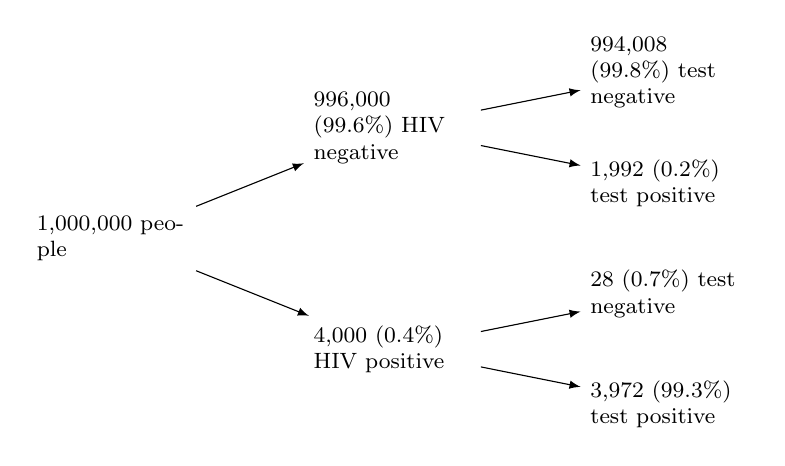
\begin{tikzpicture}
  [
    grow                    = right,
    sibling distance        = 8em,
    level distance          = 10em,
    level 2/.style          = { sibling distance=4em },
    edge from parent/.style = {draw, -latex},
    every node/.style       = {font=\footnotesize, text width=2 cm},
    sloped
  ]
  \node { 1,000,000 people }
  child {
    node { 4,000 (0.4\%) HIV positive }
    child {
      node { 3,972 (99.3\%) test positive }
    }
    child {
      node { 28 (0.7\%) test negative }
    }
  }
  child {
    node { 996,000 (99.6\%) HIV negative }
    child {
      node { 1,992 (0.2\%) test positive }
    }
    child {
      node { 994,008 (99.8\%) test negative }
    }
  };
  \end{tikzpicture}
  \pause

  Of the $3972+1992=5964$ people that tested positive, only $3972$ (66.6\%) are actually HIV positive!
  \lc
\end{frame}

\begin{frame}
  Think of Bayes' Rule as a way to update our thinking based on new information:

  \bigskip

  \begin{center}
    \begin{tabular}{ll}
      $P(HP)$ & $\longleftarrow$ Prior probability \\
      $P(HP|TP)$ & $\longleftarrow$ Posterior probability (includes new information) \\
    \end{tabular}
  \end{center}
  \lc
\end{frame}

\begin{frame}
  \fullpagepicture{doctors}
  \lc
\end{frame}

\begin{frame}
  Just 21\% of gynecologists got the right answer!
  \bigskip\pause

  In other words, this is hard, and it goes against our intuition!
\end{frame}

\begin{frame}{Example 2: Supplier detective work}
  A smartphone company assembles their phones with screens from two different suppliers. Supplier A's screens are defective at a rate of 0.5\%, and Supplier B's screens are defective at a rate of 0.3\%. (55\% of the screens are supplied by Supplier A.) Unfortunately, the shipments of screens from each supplier were not labeled and you can't tell which is which --- and there are too many to count!

  \bigskip\pause

  Suppose we draw a screen at random from one shipment and find it is defective. \pause How confident should we be that we drew from Supplier A?
\end{frame}

\begin{frame}{Example 2: Supplier detective work}
  \begin{align*}
    A &= \text{we drew from Supplier A's shipment} \\
    D &= \text{we drew a defective screen}
  \end{align*}

  \pause
  What are we looking for?
  \pause
  $P(A|D)$
  \bigskip\pause

  What is:
  \begin{itemize}
    \item $P(A) = \pause 0.55$
    \item $P(D|A) = \pause 0.005$
    \item $P(D|\overline A) = \pause 0.003$
  \end{itemize}
  \pause
\end{frame}

\begin{frame}{Example 2: Supplier detective work}
  \begin{align*}
    P(A|D) &= \frac{P(D|A)P(A)}{P(D|A)P(A) + P(D|\overline A)P(\overline A)} \\
    &= \frac{(0.005)(0.55)}{(0.005)(0.55) + (0.003)(0.45)} \\
    &= 0.67
  \end{align*}
  \bigskip\pause
  We are 67\% sure that the shipment we drew from is from Supplier A.
  \lc
\end{frame}

\begin{frame}
  \fullpagepicture{monty-hall}
\end{frame}

\begin{frame}{Example 3: Monty Hall and \emph{Let's Make a Deal}}
  \begin{itemize}[<+->]
    \item Monty Hall used to host the game show \emph{Let's Make a Deal}.
    \item There are three doors: two contain a goat, and one contains...\pause \alert{a new car}!
    \item You (the contestant) select one of three doors.
    \item Without revealing what is behind the selected door, Monty opens one of the other two doors to reveal a goat.
    \item Monty then gives you a choice: keep your original door, or switch to the other (unopened) door.
  \end{itemize}
\end{frame}

\begin{frame}
  \fullpagepicture{gameplay}
\end{frame}

\begin{frame}
  \fullpagepicture{car}
\end{frame}

\begin{frame}
  \fullpagepicture{goat}
\end{frame}

\begin{frame}{Example 3: Monty Hall and \emph{Let's Make a Deal}}
  Do you have a better chance of getting the car by switching, or by keeping your original selection---or does it not matter?
  \lc
\end{frame}

\begin{frame}{Example 3: Monty Hall and \emph{Let's Make a Deal}}
  Let's suppose we open Door 1, and Monty shows us a goat behind Door 2. We have to decide: switch to Door 3, or keep our original choice of Door 1?
  \begin{align*}
    D3 &= \text{The car is behind Door 3} \\
    G2 &= \text{Monty shows us a goat behind Door 2}
  \end{align*}

  So we want to figure out $P(D3|G2)$. What is:
  \begin{itemize}[<+->]
    \item $P(D3) = \pause 1/3$ (the car is placed randomly)
    \item $P(G2|D3) = \pause 1$ (we already picked Door 1, and Monty can't show us the car, so he has to show us the goat behind Door 2)
    \item $P(G2|\overline{D3}) = \pause 1/2$ (the car must be behind Door 1 or 2; we'll see the goat behind Door 2 only if the car is behind Door 1)
  \end{itemize}
\end{frame}

\begin{frame}{Example 3: Monty Hall and \emph{Let's Make a Deal}}
  \begin{align*}
    P(D3|G2) &= \frac{ P(G2|D3)P(D3) }{ P(G2|D3)P(D3) + P(G2|\overline{D3})P(\overline{D3}) } \\
    &= \frac{ 1 \cdot \dfrac 1 3 }{ 1 \cdot \dfrac 1 3 + \dfrac 1 2 \cdot \dfrac 2 3 } \\
    &= \frac 2 3
  \end{align*}
  \pause

  So it is \emph{better to switch} --- you have a 2/3 chance of winning if you switch!
\end{frame}

\end{darkframes}
\end{document}
